\documentclass[12pt,twoside]{report}

%%%%%%%%%%%%%%%%%%%%%%%%%%%%%%%%%%%%%%%%%%%%%%%%%%%%%%%%%%%%%%%%%%%%%%%%%%%%%

% Definitions for the title page
% Edit these to provide the correct information
% e.g. \newcommand{\reportauthor}{Timothy Kimber}

\newcommand{\reporttitle}{Learning Rules of Board Games using Answer Set Programming}
\newcommand{\reportauthor}{Luca Grillotti}
\newcommand{\supervisor}{Krysia Broda}
\newcommand{\degreetype}{Computing Science / Artificial Intelligence}

%%%%%%%%%%%%%%%%%%%%%%%%%%%%%%%%%%%%%%%%%%%%%%%%%%%%%%%%%%%%%%%%%%%%%%%%%%%%%


% load some definitions and default packages
%%%%%%%%%%%%%%%%%%%%%%%%%%%%%%%%%%%%%%%%%
% University Assignment Title Page 
% LaTeX Template
% Version 1.0 (27/12/12)
%
% This template has been downloaded from:
% http://www.LaTeXTemplates.com
%
% Original author:
% WikiBooks (http://en.wikibooks.org/wiki/LaTeX/Title_Creation)
%
% License:
% CC BY-NC-SA 3.0 (http://creativecommons.org/licenses/by-nc-sa/3.0/)
% 
%
%%%%%%%%%%%%%%%%%%%%%%%%%%%%%%%%%%%%%%%%%
%----------------------------------------------------------------------------------------
%	PACKAGES AND OTHER DOCUMENT CONFIGURATIONS
%----------------------------------------------------------------------------------------
\usepackage[a4paper,hmargin=2.8cm,vmargin=2.0cm,includeheadfoot]{geometry}
\usepackage{textpos}
\usepackage{natbib} % for bibliography
\usepackage{tabularx,longtable,multirow,subfigure,caption}%hangcaption
\usepackage{fncylab} %formatting of labels
\usepackage{fancyhdr} % page layout
\usepackage{url} % URLs
\usepackage[english]{babel}
%\usepackage{svg}
\usepackage{amsmath}
\usepackage{appendix}
\usepackage{graphicx}
\usepackage{dsfont}
\usepackage{epstopdf} % automatically replace .eps with .pdf in graphics
\usepackage{backref} % needed for citations
\usepackage{array}
\usepackage{latexsym}
\usepackage[pdftex,pagebackref,hypertexnames=false,colorlinks]{hyperref} % provide links in pdf
\usepackage{makecell}
\usepackage{fancyvrb}
\usepackage{color}
\usepackage[dvipsnames]{xcolor}


\hypersetup{pdftitle={},
  pdfsubject={}, 
  pdfauthor={},
  pdfkeywords={}, 
  pdfstartview=FitH,
  pdfpagemode={UseOutlines},% None, FullScreen, UseOutlines
  bookmarksnumbered=true, bookmarksopen=true, colorlinks,
    citecolor=black,%
    filecolor=black,%
    linkcolor=black,%
    urlcolor=black}

\usepackage[all]{hypcap}

\usepackage{amsthm}
\usepackage{verbatim}
\theoremstyle{definition}

%\usepackage{color}
%\usepackage[tight,ugly]{units}
%\usepackage{float}
%\usepackage{tcolorbox}
%\usepackage[colorinlistoftodos]{todonotes}
% \usepackage{ntheorem}
% \theoremstyle{break}
\newtheorem{lemma}{Lemma}[section]
\newtheorem{theorem}{Theorem}[section]
\newtheorem{remark}{Remark}
\newtheorem{definition}{Definition}[section]
% \newtheorem{proof}{Proof}


%%% Default fonts
\renewcommand*{\rmdefault}{bch}
\renewcommand*{\ttdefault}{cmtt}


%%% Default settings (page layout)
\setlength{\parindent}{0em}  % indentation of paragraph

\setlength{\headheight}{14.5pt}
\pagestyle{fancy}
\renewcommand{\chaptermark}[1]{\markboth{\chaptername\ \thechapter.\ #1}{}} 

\fancyfoot[ER,OL]{\sffamily\textbf{\thepage}}%Page no. in the left on odd pages and on right on even pages
\fancyfoot[OC,EC]{\sffamily }
\renewcommand{\headrulewidth}{0.1pt}
\renewcommand{\footrulewidth}{0.1pt}
\captionsetup{margin=10pt,font=small,labelfont=bf}


%--- chapter heading

\def\@makechapterhead#1{%
  \vspace*{10\p@}%
  {\parindent \z@ \raggedright \sffamily
    \interlinepenalty\@M
    \Huge\bfseries \thechapter \space\space #1\par\nobreak
    \vskip 30\p@
  }}

%---chapter heading for \chapter*  
\def\@makeschapterhead#1{%
  \vspace*{10\p@}%
  {\parindent \z@ \raggedright
    \sffamily
    \interlinepenalty\@M
    \Huge \bfseries  #1\par\nobreak
    \vskip 30\p@
  }}

\allowdisplaybreaks



% redefine \VerbatimInput
\RecustomVerbatimCommand{\VerbatimInput}{VerbatimInput}%
{fontsize=\footnotesize,
 %
 frame=lines,  % top and bottom rule only
 framesep=2em, % separation between frame and text
 rulecolor=\color{Gray},
 %
 label=\fbox{\color{Black}data.txt},
 labelposition=topline,
 %
 %commandchars=\|\(\), % escape character and argument delimiters for
                      % commands within the verbatim
 commentchar=*        % comment character
}

% load some macros
% Here, you can define your own macros. Some examples are given below.

\newcommand{\R}[0]{\mathds{R}} % real numbers
\newcommand{\Z}[0]{\mathds{Z}} % integers
\newcommand{\N}[0]{\mathds{N}} % natural numbers
\newcommand{\C}[0]{\mathds{C}} % complex numbers
\renewcommand{\vec}[1]{{\boldsymbol{{#1}}}} % vector
\newcommand{\mat}[1]{{\boldsymbol{{#1}}}} % matrix


\date{September 2017}





\begin{document}

% load title page
% Last modification: 2015-08-17 (Marc Deisenroth)
\begin{titlepage}

\newcommand{\HRule}{\rule{\linewidth}{0.5mm}} % Defines a new command for the horizontal lines, change thickness here


%----------------------------------------------------------------------------------------
%	LOGO SECTION
%----------------------------------------------------------------------------------------


\includegraphics[width = 4cm]{./figures/imperial}\\[0.5cm] 

\center % Center remainder of the page

%----------------------------------------------------------------------------------------
%	HEADING SECTIONS
%----------------------------------------------------------------------------------------

\textsc{\Large Imperial College London}\\[0.5cm] 
\textsc{\large Department of Computing}\\[0.5cm] 

%----------------------------------------------------------------------------------------
%	TITLE SECTION
%----------------------------------------------------------------------------------------

\HRule \\[0.4cm]
{ \huge \bfseries \reporttitle}\\ % Title of your document
\HRule \\[1.5cm]
 
%----------------------------------------------------------------------------------------
%	AUTHOR SECTION
%----------------------------------------------------------------------------------------

\begin{minipage}{0.4\textwidth}
\begin{flushleft} \large
\emph{Author:}\\
\reportauthor % Your name
\end{flushleft}
\end{minipage}
~
\begin{minipage}{0.4\textwidth}
\begin{flushright} \large
\emph{Supervisor:} \\
\supervisor % Supervisor's Name
\end{flushright}
\end{minipage}\\[4cm]


%----------------------------------------------------------------------------------------
%	FOOTER & DATE SECTION
%----------------------------------------------------------------------------------------
\vfill % Fill the rest of the page with whitespace
Submitted in partial fulfillment of the requirements for the MSc degree in
\degreetype~of Imperial College London\\[0.5cm]

\makeatletter
\@date 
\makeatother


\end{titlepage}



% page numbering etc.
\pagenumbering{roman}
\clearpage{\pagestyle{empty}\cleardoublepage}
\setcounter{page}{1}

%%%%%%%%%%%%%%%%%%%%%%%%%%%%%%%%%%%%
\begin{abstract}
Your abstract.
\end{abstract}

\cleardoublepage
%%%%%%%%%%%%%%%%%%%%%%%%%%%%%%%%%%%%
%*%\section*{Acknowledgments}
%*%Comment this out if not needed.

\clearpage{\pagestyle{empty}\cleardoublepage}

%%%%%%%%%%%%%%%%%%%%%%%%%%%%%%%%%%%%
%--- table of contents
\tableofcontents 


\clearpage{\pagestyle{empty}\cleardoublepage}
\pagenumbering{arabic}
\setcounter{page}{1}

%TODO : au début de chaque section, ne pas oublier de récapituler ce de quoi je vais parler.

%TODO : parler du GDL (game describing language)

%TODO : parler des changements de code entre les .lp et .las dus aux syntaxes non acceptées ???

%TODO : give examples for everything (weak constraints, context dependant examples).

%TODO : proof that the 2-Player Game gives the right result (cf paper for Single player games)

%%%%%%%%%%%%%%%%%%%%%%%%%%%%%%%%%%%%
\chapter{Introduction}
%%%%%%%%%%%%%%%%%%%%%%%%%%%%%%%%%%%%



%%%%%%%%%%%%%%%%%%%%%%%%%%%%%%%%%%%%

\chapter{Background}

\section{Answer Set Programming (ASP)}

\subsection{Logic Program}

We will work on finite Logic Programs with rules of the form:
\begin{itemize}
\item $\leftarrow b_1, b_2, ..., b_m, \text{ not } c_1, \text{ not } c_2,...,\text{ not } c_n$ (also called \textit{constraint}).
\item $a \leftarrow b_1, b_2, ..., b_m, \text{ not } c_1, \text{ not } c_2,...,\text{ not } c_n$. This is a \textit{default} rule.
\item $l\{a_1, a_2, ..., a_p\}u \leftarrow b_1, b_2, ..., b_m, \text{ not } c_1, \text{ not } c_2,...,\text{ not } c_n$, where $l$ and $u$ are numbers such that $l \leq u$. Also, $l\{a_1, a_2, ..., a_p\}u$ is true in an Herbrand Interpretation $I$ iff $ l \leq |\{a_1, a_2, ..., a_p\}\cap I | \leq u$. This type of rule is also called \textit{choice rule}.
\end{itemize}
In all these rules, "$\text{ not }$" refers to the \textit{"negation as failure"}, and $a, a_1, a_2, ..., a_p, b_1, b_2,\\ ..., b_m, c_1, c_2, ...,  c_n$ are atoms. 

\smallskip

$a$ and $l\{a_1, a_2, ..., a_p\}u$ are called the \textit{head} of the rule, and $b_1, b_2, ..., b_m, \text{ not } c_1, \text{ not } c_2,\\..., \text{ not } c_n$ is the \textit{body} of the rule. If we call $r$ the following rule: $\alpha \leftarrow b_1, b_2, ..., b_m,\\ \text{ not } c_1, \text{ not } c_2,...,\text{ not } c_n$ where $\alpha$ is either an atom or an aggregate, then $body^+(r)=\{b_1, b_2,...,b_m \}$ and $body^-(r)=\{c_1, c_2,...,c_n \}$.

\smallskip

A \textit{literal} is an atom or the negation (by failure) of an atom.

\subsection{Stable Models (Answer Sets)}

All the programs we will consider will be \textit{safe} (as defined for Disjunctive Logic Programs in \citep{dlp_safe}). As a consequence, every program can be grounded without ambiguity.

\bigskip

Let $P$ be a logic program and $X$ be an Herbrand Interpretation of $P$. From $P$ and $X$, we can construct a new program $P^X$ called the \textit{reduct} of $P$ by applying these methods \citep{stable_semantics, law_simplified}:
\begin{itemize}
\item For every rule $r\in P$, if $X\cap body^-(r)=\emptyset$, then we remove every negative literal in $r$.
\item Otherwise, if $X\cap body^-(r)\neq\emptyset$, then we delete the whole rule.
\item We replace every constraint $ :- body$ by $\perp :- body$. Here $\perp$ is an atom that does not appear in $P$. As a consequence, $\perp$ does not belong to any Answer Set.
\item For every rule $r$ with an aggregate in the head: $l\{a_1, a_2, ..., a_p\}u \leftarrow b_1, b_2, ..., b_m$ (we suppose that we have already removed the negative literals according to the first method)
\begin{itemize}
\item if $l \leq |\{a_1, a_2, ..., a_p\}\cap X | \leq u$, we replace $r$ by all the rules in the following set: $\{ a_i \leftarrow b_1, b_2, ..., b_m | a_i \in X\}$.
\item otherwise, we replace $r$ by $\perp \leftarrow b_1, b_2, ..., b_m$
\end{itemize}
\end{itemize}

Thus, the reduct $P^X$ is a \textit{definite} logic program (which means that it does not contain any negation as failure). Definite logic programs have a unique minimal Herbrand \citep{sergot_minimal} model, that is very easy to construct. We will write $M(P^X)$ the minimal Herbrand model of $P_X$.

\smallskip

We call \textit{stable model} of $P$ every Herbrand interpretation $X$ that satisfies the relation: $X=M(P^X)$ \citep{sergot_stable_model}. Moreover, as we do not use classical negation $\neg$, we will not make a distinction between \textit{answer sets} and stable models.

\smallskip

Stable models of $P$ have more properties than its models in general: they also are \textit{minimal} (for inclusion) and \textit{supported} \citep{sergot_stable_model} (every atom in the stable model appears in a rule whose body evaluates to \textit{true}). 

\subsection{Tools}

For ASP problems, we will use some of the tools developed by the University of Potsdam: \texttt{gringo} \citep{gringo_paper}, \texttt{clasp} \citep{clasp} and \texttt{clingo} \citep{clingo_paper}. \texttt{gringo} transforms the logic program in input into an equivalent variable-free program (it is a \textit{grounder}) \citep{manual_clingo}. And \texttt{clasp} is a \textit{solver} capable of solving ground logic programs. Finally, \texttt{clingo} only combines grounding (with \texttt{gringo}) and solving (with \texttt{clasp}). 

\smallskip

We used the version 4.3.0 of \texttt{clingo} since this the one that ILASP uses.
%TODO : reference manuel

\smallskip

\begin{remark}
\texttt{gringo} (and \texttt{clingo} by extension) only works with \textit{safe} programs. \citep{manual_clingo}
\end{remark}

\subsection{Optimization in clingo}\label{subseq:optimization}

In \texttt{clingo}, it is possible to explain what kind of answer sets are optimal by using \textit{weak constraints} \citep{manual_clingo}. A weak constraint has the following form:
\begin{center}
\texttt{:$\sim$ t$_1$, t$_2$, t$_3$,..., t$_n$.[w@p, id$_1$, id$_2$, ..., id$_m$]}
\end{center}
where \texttt{w} is called the \textit{weight}, and \texttt{p} is called the \textit{priority} of the weak constraint. We will also call \textit{ID} of the weak constraint the list \texttt{[\texttt{w}, \texttt{p}, id$_1$, id$_2$, ..., id$_m$]}. We say that a weak constraint is satisfied by an answer set $A$ if there is at least one atom among t$_1$, t$_2$, t$_3$,..., and t$_n$ that is not in $A$.

\smallskip

\begin{remark}

\texttt{id$_1$}, \texttt{id$_2$}, ..., \texttt{id$_m$}, \texttt{w} and \texttt{p} can be variables. \texttt{clingo} considers that a weak constraint is safe iff any variable among those atoms appears in a positive literal in the body of the weak constraint. 

\end{remark}

\smallskip

We call cost of an answer set $A$ for a given priority \texttt{p} (written $cost_{\texttt{p}}(A)$) the sum of the weights \texttt{w} of the different lists \texttt{[\texttt{w}, \texttt{p}, id$_1$, id$_2$, ..., id$_m$]} such that: there is at least a weak constraint whose ID is  \texttt{[\texttt{w}, \texttt{p}, id$_1$, id$_2$, ..., id$_m$]} that is violated by $A$.

\bigskip

As a consequence:
\begin{itemize}
\item if we prefer the answer sets that satisfy a constraint \texttt{:- t$_1$, t$_2$, t$_3$,..., t$_n$.}, then we can use a weak constraint of the form \texttt{:$\sim$ t$_1$, t$_2$, t$_3$,..., t$_n$.[w@p, id$_1$, id$_2$, ..., id$_m$]} where the weight \texttt{w} is \textbf{positive}.
\item if we prefer the answer sets that satisfy all the atoms \texttt{t$_1$, t$_2$, t$_3$,...,} and \texttt{t$_n$} at the same time, then we can use a weak constraint of the form \texttt{:$\sim$ t$_1$, t$_2$, t$_3$,..., t$_n$.[w@p, id$_1$, id$_2$, ..., id$_m$]} where the weight \texttt{w} is \textbf{negative}.
\end{itemize}

\smallskip

For \texttt{clingo}, in a given ASP program $P$, an answer set $A_1$ \textbf{is preferred to} $A_2$ if and only if $cost_{\texttt{p}}(A_1)<cost_{\texttt{p}}(A_2)$ where \texttt{p} is the highest priority for which $cost_{\texttt{p}}(A_1)\neq cost_{\texttt{p}}(A_2)$.

\begin{example}
We consider the following ASP program:\newline
\texttt{1\{go\_on\_holidays ; work\_at\_imperial\}1.\\
bad\_mark :- go\_on\_holidays.\\
good\_mark :- work\_at\_imperial.}

\smallskip

To this program we add the two following weak constraints:\newline
\texttt{:$\sim$ go\_on\_holidays.[-1@1] \% we enjoy holidays (priority 1)\\
:$\sim$ good\_mark.[-1@2] \% we like good marks (priority 2)}

\smallskip

This ASP program has two answer sets: $A_1 = \{ \texttt{go\_on\_holidays}, \texttt{bad\_mark}\}$ and $A_2 = \{ \texttt{work\_at\_imperial}, \texttt{good\_mark} \}$. 

\begin{itemize}
\item $A_1$ satisfies only the second weak constraint. So its scores are $cost_1(A_1)=-1$ and $cost_2(A_1)=0$.
\item $A_2$ satisfies only the first weak constraint. So its scores are $cost_1(A_2)=0$ and $cost_2(A_2)=-1$.
\end{itemize}

The highest priority is 2 and $cost_2(A_2)<cost_2(A_1)$. Thus, $A_2=\{ \texttt{work\_at\_imperial}, \texttt{good\_mark} \}$ is optimal, even if $cost_1(A_2)>cost_1(A_1)$.
\end{example}

\section{Single-Player Games in ASP}

%TODO : parler ici de GDL c'est quoi + ref 
%TODO : stratified imposed by GDL

With Game Description Language (GDL) \citep{gdl}, it is possible to describe finite games with any number of players by using logical facts and rules, that describe respectively the states and mechanics of the tame.

\smallskip

On the basis of GDL, \citep{thielscher2009answer} explains how to describe any finite single-player game in Answer Set Programming (ASP) and how to use \texttt{clingo} to simulate a game play.

\smallskip

To illustrate the predicates that can be used to describe the games under study, we will focus on a basic example: a simple graph game. After having explained the rules of the game, we will \textbf{describe} it in ASP, and then, we will add some rule in order to \textbf{simulate} a game play.

\subsection{Rules of the game}

The rules of the graph game on figure \ref{fig:agent} are the following:
\begin{itemize}
\item The player starts in state $a$.
\item If the player is in state $a$ or in state $b$ then he can go to the left or to the right.
\item The player wins iff he goes to the state \textit{"victory"}.
\item The player cannot go back to state $a$ once he has reached the state \textit{"hole"}.
\end{itemize}

\begin{figure}[h]
\centering
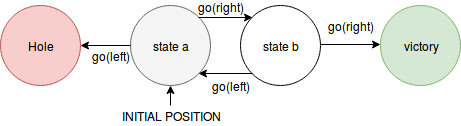
\includegraphics[width = 0.8\hsize]{figures/diagram1.png}
\caption{Simple graph game}
\label{fig:agent}
\end{figure}

\subsection{Describing the game in ASP}
\label{subsection:asp_description}
\begin{itemize}

\item We start by defining the different players in the game by using the predicate \texttt{role}. Here, there is only one player so we include the fact: \texttt{role(player).}

\smallskip

\item Then, we define what are the initial states by using the predicate \texttt{holds} for the first time-step:\newline
\texttt{holds(hole, empty, 1).}\\
\texttt{holds(a, player, 1).} \% the player is in state $a$\\
\texttt{holds(b, empty, 1).}\\
\texttt{holds(victory, empty, 1).}

\item We also say what actions are legal at time $T$, depending on the state the player is:\newline
\texttt{legal(player,go(left),T) :- holds(a,player,T) ; holds(b,player, T)}\\
\texttt{legal(player,go(right),T) :- holds(a,player,T) ; holds(b,player,T)}

\item And we explain the situation at time $T+1$ depends on what holds at time $T$ and what the player does:\newline
\texttt{holds(hole,player,T+1) :- holds(a,player,T), does(player,go(left),T).}\\
\texttt{holds(b,player,T+1) :- holds(a,player,T), does(player,go(right),T).}\\
\texttt{...}

\item We can also define what is a \texttt{terminal} state, and we can evaluate each final state by using the predicate \texttt{goal}: \newline
\texttt{terminal(T) :- holds(victory, player, T).}\\
\texttt{terminal(T) :- holds(hole, player, T).}\\
\texttt{goal(player,100,T) :- holds(victory, player, T).}\\
\texttt{goal(player,  0,T) :- holds(hole, player, T).}
\end{itemize}

All these rules are \textbf{describing} the game in ASP.

\bigskip

We will respect the following Game Description Language (GDL) restrictions: as long as we \textbf{describe} the game in ASP (and do not want to \textbf{simulate} a game play), the predicate \texttt{does} only appears in rule bodies, and does not appear in the definition of \texttt{terminal}, \texttt{goal} or \texttt{legal}. Besides, a GDL game must be \textit{stratified} \citep{stratified, gdl}. But if \texttt{not holds(P, A, T)} appears in the definition of \texttt{holds(P, action\_1, T+1)}, there will not be any problem with the description or the simulation of the game. That is why our Answer Sets Programs for game description will be \textit{locally stratified} \citep{locally_stratified}

\subsection{Finding a solution to the game/Simulating a gameplay}
\label{subsection:simulate}
We have just defined a few predicates to translate the rules of the game in ASP. Now we want to \textbf{simulate} a game play and find winning sequences of moves.
\begin{itemize}
\item First of all, the player can do only one move at every time step (as long as the game is not finished).\newline
\texttt{1\{does(player,go(left),T);does(player,go(right),T)\}1 :- not terminated(T).}\\
Where \texttt{terminated(T)} is true if and only if there is a T1 such that $T1<T$ and \texttt{terminal(T1)} is true:\newline
\texttt{terminated(T) :- terminal(T).}  \\
\texttt{terminated(T+1) :- terminated(T).}

\item Also, every move that is played must be legal:\newline
\texttt{:- does(player, M, T), not legal(player, M, T).}

\item We want the game to terminate at some point:\newline
\texttt{:- 0\{terminated(T) : time\_domain(T)\}0.}\\
\texttt{time\_domain(1..10). \% We allow at most 10 moves} 

\item Finally, we would like to find a sequence of moves in order to win the game:\newline
\texttt{:- terminal(T), not goal(player, 100, T)}

\end{itemize}

\colorbox{yellow}{TO DO: an ASP solution ?}

\section{Inductive Logic Programming}

In this part, $B$ is the logic program that represents the \textit{Background Knowledge}, $S_M$ is the set of possible hypotheses, $E^+$ is the set of positive examples (all the elements that have been observed) and $E^-$ is the set of negative examples (all the elements that can't appear in any result). Our task is to find an hypothesis $H\in S_M$ such that $B\cup H$ \textit{explains} $E^+$ and $E^-$. There are different ways of defining the word "explains" used in the last sentence. We will have a look at three of them.

%TODO S_M ???

\subsection{Brave Inductive Logic Programming}

\subsubsection{Brave Induction}

\begin{definition}

A \textit{brave inductive task} is a tuple $T_b=<B, S_M, E^+, E^->$ where $E^+$ and $E^-$ are sets of atoms occurring in the Herbrand Base of $B$. 

\smallskip

A hypothesis $H$ is solution of $T_b$ iff there is an answer set $A$ of $B\cup H$ verifying $E^+\subseteq A$ and $E^-\cap A = \emptyset$

\smallskip

We call $ILP_b(B,E^+,E^-)$ the set of hypotheses that are solutions of $T_b$. 

\end{definition}

\subsubsection{ASPAL encoding}

By using ASPAL \citep{aspal}, we can find the optimal solutions to a brave inductive task. We illustrate how to use ASPAL encoding with \texttt{clingo} in the following example.\bigskip

First of all, we consider the background knowledge $B$:\newline
\texttt{person(Nicolas). person(Pierre).\\
play\_video\_games(Nicolas). play\_video\_games(Pierre). works(Nicolas).}\\

And we take: $E^+=\{\texttt{good\_marks(Nicolas)}\}$ and $E^-=\{\texttt{good\_marks(Pierre)}\}$

\begin{itemize}
\item We are studying the hypotheses that are following this mode: \texttt{modeh(good\_marks(+X))}, \texttt{modeb(1,works(+X))} and \texttt{modeb(1,play\_video\_games(+X))}. So we write all the possible hypotheses, and we add the predicate rule/1 that takes as an argument the id of the hypothesis.\newline
\texttt{good marks(P) :- person(P), rule(1).\\
good\_marks(P) :- person(P), works(P), rule(2).\\
good\_marks(P) :- person(P), play\_video\_games(P), rule(3).\\
good\_marks(P) :- person(P), works(P), play\_video\_games(P), rule(4).}

\item We will select some rules between those above:\newline
\texttt{0\{rule(1..4).\}4}

\item And we want to respect the examples:\newline
\texttt{goal :- good\_marks(Nicolas), not good\_marks(Pierre).\\
:- not goal.}

\item Finally, we want to find the optimal (the shortest) hypothesis:\newline
\texttt{:$\sim$ rule(1).[2@1] \% the weight denotes the length of the rule\\
:$\sim$ rule(2).[3@1]\\
:$\sim$ rule(3).[3@1]\\
:$\sim$ rule(4).[4@1]\\}
\end{itemize}

\texttt{clingo} finds three answer sets for the new ASP program:
\begin{itemize}
\item The first one $A_1$ contains \texttt{rule(2)}, and \texttt{rule(i)}$\not \in A_1$ for $\texttt{i}\neq 2$. Also, \texttt{rule(2)} denotes the following hypothesis: $H_1=\{\texttt{good\_marks(P) :- person(P), works(P).}\}$. So $H_1\in ILP_b(B,E^+,E^-)$. Moreover, as  \texttt{rule(2)} appears in the body of the second weak constraint, $cost_{1}(A_1)=3$ (see \ref{subseq:optimization}).

\item The second answer set $A_2$ only contains \texttt{rule(4)}, which denotes \\$H_2=\{$\texttt{good\_marks(P) :- person(P), works(P), play\_video\_games(P).}$\}$. As a consequence, $H_2\in ILP_b(B,E^+,E^-)$, and $cost_{1}(A_2)=4$.

\item The third answer set $A_3$ contains both \texttt{rule(2)} and \texttt{rule(4)}. As a consequence, $H_1\cup H_2 \in ILP_b(B,E^+,E^-)$, and $cost_{1}(A_3)=7$.

\end{itemize} 

As $cost_{1}(A_1)<cost_{1}(A_2)<cost_{1}(A_3)$ (see \ref{subseq:optimization}), the optimal answer set is $A_1$, which means that the optimal (shortest in this case) hypothesis is $H_1$. 

\bigskip

We have just seen that with the ASPAL encoding, we can find an hypothesis for which \textit{there is} an answer set respecting all the positive and negative examples. However, it is not able to find a solution to a \textit{cautious inductive task}. 

\subsection{Cautious Inductive Logic Programming}

\begin{definition}

A \textit{cautious inductive task} is a tuple $T_c=<B, E^+, E^->$ where $E^+$ and $E^-$ are sets of atoms occurring in the Herbrand Base of $B$.

\smallskip

A hypothesis $H$ is solution of $T_c$ iff 
\begin{itemize}
\item $B\cup H$ has at least one answer set
\item every answer set of $B\cup H$ verifies $E^+\subseteq A$ and $E^-\cap A = \emptyset$
\end{itemize}

\smallskip

We call $ILP_c(B,E^+,E^-)$ the set of hypotheses that are solutions of $T_c$. 

\end{definition}

%TODO pas possible avec clingo

\subsection{Inductive Learning From Answer Sets Programming}

We present here a new type of inductive task which is more general than the cautious and the brave inductive tasks. All the definitions and remarks in this subsection are based on \citep{law2014inductive, law2015weak, law2016context} and were reformulated as much as possible for this report. Nevertheless, all the examples were created by us.

\subsubsection{Partial Interpretations}

\begin{definition}[\citep{law2014inductive}]
We call \textit{partial interpretation} a tuple $<e^+,e^->$ where $e^+=\{e^+_1,e^+_2,...,e^+_m\}$ and $e^-=\{e^-_1,e^-_2,...,e^-_n\}$ are two sets of atoms. 

\smallskip

We say that an interpretation $I$ of $B$ extends a partial interpretation $<e^+,e^->$ iff $e^+ \subseteq I$ and $e^- \cap I = \emptyset$.
\end{definition}

\subsubsection{Learning from Answer Sets Induction}

\begin{definition}[\citep{law2014inductive}]

A \textit{Learning from Answer Sets task} is a tuple $T_{LAS}=<B, S_M, E^+, E^->$ where $S_M$ is the hypothesis space; and $E^+$ and $E^-$ are sets of partial interpretations. 

\smallskip

An hypothesis $H$ is solution of $T_{LAS}$ iff 
\begin{itemize}
\item $H\subseteq S_M$
\item For all  $<e^+,e^->\in E^+$, there is an answer set of $B\cup H$ that extends $<e^+,e^->$
\item For all  $<e^+,e^->\in E^-$, there are no answer sets of $B\cup H$ that extend $<e^+,e^->$
\end{itemize}

We call $ILP_{LAS}(B,S_M,E^+,E^-)$ the set of hypotheses that are solutions of $T_{LAS}$. 
\end{definition}

\begin{example}

For example, we consider the following background knowledge $B$:

\texttt{student(Nicolas). \% Nicolas works and sleeps\\
works(Nicolas).\\
sleeps(Nicolas).\\
\\
student(Pierre). \% Pierre only works\\
works(Pierre). \\
\\
student(Jean). \% Jean only sleeps\\
sleeps(Jean). \\
\\
1\{good\_mark(P); bad\_mark(P)\}1 :- student(P). \% a student can have a either \\
											\% a good or a bad mark}
											
with the following hypothesis space $S_M$: \\
$\{$ \texttt{good\_mark(P) :- student(P).\\
good\_mark(P) :- student(P), sleeps(P).\\
good\_mark(P) :- student(P), works(P).\\
good\_mark(P) :- student(P), works(P), sleeps(P).} $\}$\\
and the following positive and negative examples: \\$E^+=\{<\{\texttt{bad\_mark(pierre),bad\_mark(jean)}\},\emptyset>\}$ \\and $E^-=\{<\{\texttt{bad\_mark(nicolas)}\},\emptyset>\}$.

\bigskip

First, $\emptyset$ is not a valid solution, as $\emptyset\cup H$ has an answer set which contains $\texttt{bad\_mark(nicolas)}$ and which consequently extends the negative example. With the first hypothesis, there is an answer set that satisfies the positive example, but there is also an answer set that extends the negative example. With the next two hypotheses, there are no answer sets that satisfy the negative example, but the positive example is never satisfied. With the last hypothesis, Nicolas is sure to have a good grade (the negative example is not extended by any answer set), and there is an answer set that contains both \texttt{bad\_mark(pierre)} and \texttt{bad\_mark(jean)}.

\bigskip

Thus $ILP_{LAS}(B,S_M,E^+,E^-)=\{\texttt{good\_mark(P) :- student(P), works(P), sleeps(P).}\}$

\end{example}

\begin{remark}
Every brave or cautious inductive task is a Learning from Answer Sets task \citep{law_notes}. But the inverse is not true.

%TODO : reference paper
%TODO : proof ? in appendix ?

\end{remark}

\begin{proof}

\proofpart{1}{A brave inductive task is a Learning from Answer Sets task}
We consider the following brave inductive task: $T_b=<B,S_M,$ $\{e^+_1, e^+_2,...,e^+_m\},$ $\{e^-_1,...,e^-_n\}>$, and the following Learning from Answer Sets task: $T_{LAS}=<B,S_M,$ $\{p^+\},$ $\emptyset>$ where $p^+=<\{e^+_1, e^+_2,...,e^+_m\},$ $\{e^-_1,...,e^-_n\}>$.

\smallskip

\begin{tabular}{cc}
An hypothesis $H$ is solution of $T_{LAS}$ iff & \makecell[tl]{ $H\subseteq S_M$ and there is an answer set $A$ of\\ $B\cup H$ such that $A$ extends $p^+$}\\\\
\makecell[r]{iff} & \makecell[tl]{ $H\subseteq S_M$ and there is an answer set $A$ of\\ $B\cup H$ such that $A$ extends $p^+$}\\\\
\makecell[r]{iff} & \makecell[tl]{ $H\subseteq S_M$ and there is an answer set $A$ of\\ $B\cup H$ that contains all the $e^+_i$ and that \\does not contain any of the  $e^-_i$}\\\\
\makecell[r]{iff} & \makecell[tl]{ $H$ is solution of $T_b$}
\end{tabular}

\bigskip

So, the two tasks $T_b$ and $T_{LAS}$ are equivalent. Thus, we can construct a Learning from Answer Sets task from every brave inductive task.
 
\proofpart{2}{A cautious inductive task is a Learning from Answer Sets task}
 
We consider the following cautious inductive task: $T_c=<B,S_M,$ $\{e^+_1, e^+_2,...,e^+_m\},$ $\{e^-_1,...,e^-_n\}>$, and the following Learning from Answer Sets task: $T_{LAS}=<B,S_M,\emptyset,$ $\{p^-_1,...,p^-_m, q^-_1,...,q^-_n\}>$ where where for all $i$, $p^-_i=<\emptyset,\{e^+_i\}>$ and $q^-_i=<\{e^-_i\},\emptyset>$.

\smallskip

We can notice that an answer set $A$ extends $p^-_i$ iff $e^+_i\not \in A$. In addition, $A$ extends $q^-_i$ iff $e^-_i \in A$.

\smallskip

\begin{tabular}{cc}
\makecell{An hypothesis $H$ is solution of $T_{LAS}$ iff} & \makecell[lt]{ $H\subseteq S_M$ and for every answer set $A$ of\\ $B\cup H$, $A$ does not extend $p^-_i$ and $q^-_i$\\ (for all $i$)}\\\\
\makecell[r]{iff} & \makecell[tl]{$H\subseteq S_M$ and for every answer set $A$ of\\ $B\cup H$, $A$ contains $e^+_i$ and \\does not contain $e^-_i$ (for all $i$)}\\\\
\makecell[r]{iff} & \makecell[tl]{ $H$ is solution of $T_c$}\\
\end{tabular}

\bigskip

So, the two tasks $T_c$ and $T_{LAS}$ are equivalent. Thus, we can construct a Learning from Answer Sets task from every cautious inductive task.

\end{proof}

\subsubsection{Learning from Ordered Answer Sets}

The definition of Learning from Answer Sets task can be extended to take into account the ordering relations between the different answer sets of the ASP program \citep{law2015weak}. We will first define what is an ordering example, and how it can be used to represent the ordering relations.

\begin{definition}[\citep{law2015weak}]

We will call \textit{ordering example} every pair $<e_1,e_2>$ of partial interpretations. These are two ways for an ASP program to cover an ordering example:
\begin{itemize}
\item An ordering example is \textit{bravely covered} by an ASP program $P$ iff \textbf{there are} two answer sets $A_1$ and $A_2$ such that $A_1$ extends $e_1$, $A_2$ extends $e_2$ and $A_1$ is preferred to $A_2$.
\item An ordering example is \textit{cautiously covered} by an ASP program $P$ iff \textbf{for every} answer sets $A_1$ and $A_2$ such that $A_1$ extends $e_1$ and $A_2$ extends $e_2$ we have : $A_1$ is preferred to $A_2$.
\end{itemize}
\end{definition}

Now we can give the definition for a Learning from Ordered Answer Sets task \citep{law2015weak}:

\begin{definition}
A \textit{Learning from Ordered Answer Sets task} is a tuple $T_{LOAS}=<B, S_M, E^+, E^-,O^{brave}, O^{cautious}>$ (where $<B,S_M, E^+, E^->$ is a Learning from Answer Sets task, and $O^{brave}$ and $O^{cautious}$ are sets of ordering examples) such that: every partial interpretation that appears in $O^{brave}$ and $O^{cautious}$ is in $E^+$.

\smallskip

A hypothesis $H$ is solution of $T_{LOAS}$ iff 
\begin{itemize}
\item $H$ is a solution of $T_{LAS}=<B, S_M, E^+, E^->$.
\item Every ordering example in $O^{brave}$ is bravely covered by $B\cup H$
\item Every ordering example in $O^{cautious}$ is cautiously covered by $B\cup H$
\end{itemize}

We call $ILP_{LOAS}(B,S_M,E^+,E^-,O^{brave},O^{cautious})$ the set of hypotheses that are solutions of $T_{LOAS}$.
\end{definition}

\begin{example}
The week preceding an exam, a student has to decide if he will work or not. And at the end, he will get a mark that is good or not: $B=\{\texttt{0\{works\}1. 
0\{good\_mark\}1.}\}$

\bigskip

We define three positive examples: $e_1 = <\{\texttt{good\_mark}\},\{\texttt{works}\}>$, $e_2 = <\{\texttt{good\_mark},\texttt{ works}\},\emptyset>$ and $e_3 = <\emptyset,\{\texttt{good\_mark}\}>$. $E^+=\{e_1, e_2, e_3\}$. Besides, we take $E^-=\emptyset$.

\bigskip

Now we define the student's preferences:
\begin{itemize}
\item For him, having a good mark without working is better than having a good mark by working hard: $O^{brave}=\{<e_1,e_2>\}$
\item The student always prefers having a good grade without working than having a bad grade: $O^{cautious}=\{<e_1,e_3>\}$
\end{itemize}

Finally, we define the hypothesis space $S_M$:\\
$\{$ \texttt{:$\sim$ not works.[-1@1]\\
:$\sim$ good\_mark.[-1@1]\\
:$\sim$ not works, good\_mark.[-1@1]} $\}$\\

\bigskip

With the first hypothesis only, the answer set $A_1=\{$\texttt{good\_mark}$\}$ extends $e_1$, and $A_3=\emptyset$ is an other answer set that extends $e_3$. In this case, $cost_1(A_1)=cost_1(A_3)=-1$, so the ordering example in $O^{cautious}$ is not cautiously covered.

\bigskip

With the second hypothesis only, the only answer set that extends $e_1$ is $A_1=\{$\texttt{good\_mark}$\}$, and $A_2=\{$\texttt{good\_mark}$,$ \texttt{works}$\}$ is the only answer set that extends $e_2$. In this case, $cost_1(A_1)=cost_1(A_2)=-1$, so the ordering example in $O^{brave}$ is not bravely covered.

\bigskip

The last hypothesis respects all the brave and cautious orderings. Indeed $cost_1(A_1)=-1$ whereas for every answer set $A$ different form $A_1$, we have: $cost_1(A)=0$. But this is not the only hypothesis in $ILP_{LOAS}(B,S_M,E^+,E^-)$, as $H=\{$\texttt{:$\sim$ not works.[-1@1], :$\sim$ good\_mark.[-1@1]}$\}$ is also a solution (of length 2).

\bigskip

To conclude \texttt{:$\sim$ not works, good\_mark.[-1@1]} is \textbf{an} optimal (shortest) hypothesis of  $ILP_{LOAS}(B,S_M,E^+,E^-)$

\end{example}

\subsubsection{Learning from Context Dependant Answer Sets}
%TODO : talk about ILASP --2i

The task defined above can be generalized by adding a \textit{context} to every partial interpretation \citep{law2016context}. A \textit{context} is an ASP program that does not contain any weak constraint or any other statement used to classify answer sets. Instead of containing partial interpretations, $E^+$ and $E^-$ contain tuples $<<e^+,e^->,C>$ where $<e^+,e^->$ is a partial interpretation, and $C$ is the \textit{context} of this partial interpretation. 

\bigskip

As the definitions of positive and negative examples have been generalized by adding contexts, we need to extend the definition of an ordering example \citep{law2016context}.

\begin{definition}

We will call \textit{Context-Dependant Ordering Example} every pair $<<e_1,C_1>,<e_2,C_2>>$ where $e_1$ and $e_2$ are partial interpretations, and $C_1$ and $C_2$ are respectively the contexts of $e_1$ and $e_2$. These are two ways for an ASP program to cover an ordering example:
\begin{itemize}
\item An ordering example is \textit{bravely covered} by an ASP program $P$ iff \textbf{there is} an answer set $A_1$ of $P\cup C_1$ and \textbf{there is} an answer set $A_2$ of $P\cup C_2$ such that $A_1$ extends $e_1$, $A_2$ extends $e_2$ and $A_1$ is preferred to $A_2$.
\item An ordering example is \textit{cautiously covered} by an ASP program $P$ iff \textbf{for every} answer set $A_1$ of $P\cup C_1$ and \textbf{every} answer set $A_2$ of $P\cup C_2$ such that $A_1$ extends $e_1$ and $A_2$ extends $e_2$, we have: $A_1$ is preferred to $A_2$.
\end{itemize}

\end{definition}
%TODO : coverage ????
Now that we have a definition for Context-Dependant Ordering Examples, for brave coverage and for cautious coverage, the \textit{Learning from Context Dependant Answer Sets task} can be defined.

\begin{definition}[\citep{law2016context}]
A \textit{Learning from Context Dependant Answer Sets task} is a tuple $T_{LOAS}^{Context}=<B, S_M, E^+, E^-,O^{brave}, O^{cautious}>$, where $S_M$ is the hypothesis space; $E^+$ and $E^-$ are sets of tuples $<<e^+,e^->,C>$ containing a partial interpretation $<e^+,e^->$ and a context $C$; and $O^{brave}$ and $O^{cautious}$ are sets of ordering examples such that: every partial interpretation that appears in $O^{brave}$ and $O^{cautious}$ is in $E^+$.

\smallskip

A hypothesis $H$ is solution of $T_{LOAS}$ iff 
\begin{itemize}
\item $H\subseteq S_M$
\item $\forall <<e^+,e^->,C>\in E^+$, there is an answer set of $B\cup H \cup C$ that extends $<e^+,e^->$
\item $\forall <<e^+,e^->,C>\in E^-$, there is no answer set of $B\cup H \cup C$ that extends $<e^+,e^->$
\item Every ordering example in $O^{brave}$ is bravely covered by $B\cup H$
\item Every ordering example in $O^{cautious}$ is cautiously covered by $B\cup H$
\end{itemize}

We call $ILP_{LOAS}^{Context}(B,S_M,E^+,E^-,O^{brave},O^{cautious})$ the set of hypotheses that are solutions of $T_{LOAS}^{Context}$.
\end{definition}

\begin{example}
We consider a student in three different contexts: the empty context ($C_1=\emptyset$), during exams ($C_2=\{\texttt{exams}\}$) and during exams when the student is exhausted ($C_3=\{\texttt{exams, exhausted}\}$).

\bigskip

When the context is empty, the student sometimes does not study. So $e^+_1=<<\emptyset, \{\texttt{study}\}>,C_1>$ is a positive example. Moreover, if he is exhausted and in a period of exams, he is not always able to study. As a consequence, $e^+_2=<<\emptyset, \{\texttt{study}\}>,C_3>$ is an other positive example. We take $E^+=\{e^+_1,e^+_2\}$.

\bigskip

Besides, this student always works for exams (except in exceptional cases). Thus $e^-=<<\emptyset, \{\texttt{study}\}>,C_2>$ is a negative example. And we take $E^-=\{e^-\}$.

\bigskip

We choose to study $ILP_{LOAS}^{Context}(B, S_M, E^+, E^-, \emptyset, \emptyset)$ where $B=\emptyset$ and the hypothesis space $S_M$ is:\\
$\{$ \texttt{study.\\
study :- exams.\\
study :- not exhausted.\\
study :- exams, not exhausted.} $\}$

\bigskip

First of all, $\emptyset$ is not a valid hypothesis, as $B\cup \emptyset \cup C_2$ has only one answer set $\{\texttt{exams}\}$ and it does not contain \texttt{study} ($e^-$ is not respected). 

\bigskip

Then, with the first hypothesis (called $H_1$), the student would study every time (even during exams), so the negative example $e^-$ is covered. However, $B \cup H_1 \cup C_1$ has only one answer set: $\{\texttt{study}\}$ so the first positive example $e^+_1$ is not respected. 
	
\bigskip

According to the second hypothesis $H_2=\{\texttt{study :- exams.}\}$, the student studies if there is an exam, so $e^-$ is once again respected. In addition, $\emptyset$ is the unique answer set of $B\cup H_2 \cup C_1$, which proves that $e^+_1$ is respected this time. But $B\cup H_2 \cup C_3$ has only one answer set: $\{\texttt{study, exams, exhausted}\}$ and it does not extend the partial interpretation in $e^+_2$. As a consequence, the positive example $e^+_2$ is not covered.

\bigskip

With the third hypothesis $H_3$, the second positive example $e^+_2$ is covered, but the first one $e^+_1$ is not. Indeed, the unique answer set of $B\cup H_3 \cup C_1$ is$\{\texttt{study}\}$ and it does not extend $<\emptyset, \{\texttt{study}\}>$.

\bigskip

Finally, with the last hypothesis, all the positive and negative examples are respected. Besides, every union of 2 or more rules in $S_M$ does not cover all the positive examples. So $\{$\texttt{study :- exams, not exhausted.}$\}$ is the only valid hypothesis. Thus, $ILP_{LOAS}^{Context}(B, S_M, E^+, E^-, \emptyset, \emptyset) = \{\:\{\texttt{study :- exams, not exhausted.}\}\:\}$

\end{example}

\subsubsection{ILASP}

ILASP is a tool developed at Imperial College London that is capable of finding the optimal hypothesis for Learning from Context Dependent Answer Sets tasks . We only need to give it: the background knowledge with the \texttt{clingo} syntax, and the mode declaration for the variables that can appear in the head or in the body of a rule in the hypothesis. We can also specify the positive and negative partial interpretations of the task. By default, ILASP considers that the optimal hypothesis is the one that contains the least number of atoms.

\paragraph{Learning rules of games/environment}

ILASP has been used for learning the rules of Sudoku. Also, a simulated agent in an unknown environment could learn progressively the rules of this environment (such that: ”the agent cannot go through a wall”, ”the agent has to get the key before entering a locked cell”...).

\paragraph{Learning weak constraints}

ILASP can also be used to solve Learning from Ordered Answer Sets tasks.

%TODO : cite second paper from Mark

\smallskip

Do to so, we specify the partial interpretations that belong to $E^+$ and we give them names (like \texttt{pos1}, \texttt{pos2}...). Then we can define the ordering examples and we declare if we want them to be bravely or cautiously covered. 

\smallskip

Moreover, the maximal priority of the weak constraints in the hypothesis space and the their weight can be adjusted.

\smallskip

ILASP can find the optimal (with the least number of atoms by default) weak constraint that respects the declaration mode and that satisfies all the orderings.
%\begin{itemize}
%\item If we want $<\texttt{pos1},\texttt{pos2}>$ to be bravely covered by the program, we write \texttt{\#brave\_ordering(pos1, pos2).}
%\item If we want $<\texttt{pos1},\texttt{pos2}>$ to be cautiously covered by the program, we write \texttt{\#cautious\_ordering(pos1, pos2).}
%\end{itemize} 

\paragraph{Learning from Context Dependant Answer Sets} 

We can add a context to every positive or negative example, ILASP is capable of finding the optimal solution of a Learning from Context Dependant Answer Sets task.

\paragraph{Learning from Noisy Examples}

ILASP (v3) is also able to learn from noisy data: it can learn an hypothesis that covers a majority (or the most important) examples. To do so, we need to specify which examples are in the noisy data, and we give a weight to them. 

\smallskip

Then, ILASP will minimize the sum of the length of the hypothesis and of the weights of the uncovered examples (the weight of an example reflects its importance).

%TODO : décrire l'algo utilisé par ILASP ? Ou comparaison des différentes version d'ILASP sur le fonctionnement de l'algo
%TODO : 




\chapter{From Single Player Games to Two Player Games}

\section{Games under study}

This project focuses on three games: \textit{Five Field Kono}, \textit{Nine Men's Morris} and \textit{ASALTO}.

\bigskip

\subsection{Five Field Kono}

%TODO : describe origin/ rules/ etc...
Five Field Kono is a Korean strategy game. It is played on a $5\times 5$ grid. Its initial configuration is as presented in figure \ref{fig:FFK_initial}. 

\begin{figure}[h]
\centering
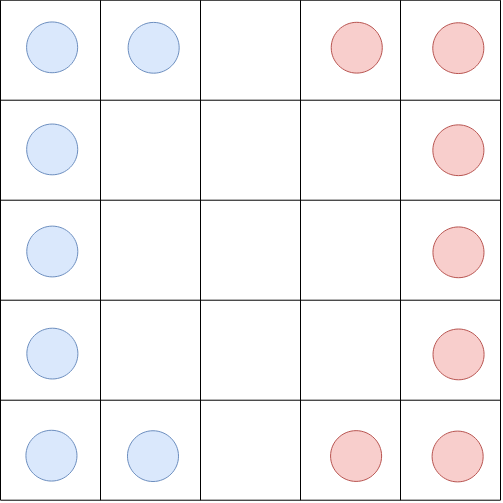
\includegraphics[width = 0.3\hsize]{figures/FFK_rules.png}
\caption{Initial configuration of Five Field Kono. The two players (in blue and red) have seven pawns each.}
\label{fig:FFK_initial}
\end{figure}

The two opponents move one of their pawns in turn knowing that a pawn can only be moved diagonally to an adjacent square (forwards or backwards). A player wins if all his pawns have taken the positions initially held by his opponent's pawns (see figure \ref{fig:FFK_ending}).

\begin{figure}[h]
\centering
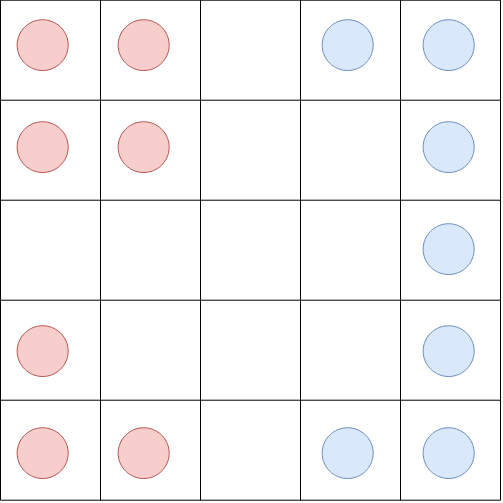
\includegraphics[width = 0.3\hsize]{figures/FFK_ending.png}
\caption{Situation where the blue player wins at Five Field Kono. Every blue pawn is in a square initially occupied by a red pawn (see figure \ref{fig:FFK_initial})}
\label{fig:FFK_ending}
\end{figure}


\subsection{Nine Men's Morris}

Nine Men's Morris is also a Korean strategy game \citep{9MM_rules}. At first the two opponents place in turn their pawns on the board (figure \ref{fig:9MM_initial}). When three pawns are aligned on the board, we say that they form a \textbf{mill}. Each time a player does a mill, he can remove one of his opponent's pawns on the board (that is not already in a mill if possible). Once both players have placed all their pawns, they move in turn one of them to an adjacent empty position. In this second phase, creating a meal has the same effect as before. A player wins if his opponent cannot move or has only two pawns left.

\begin{figure}[h]
\centering
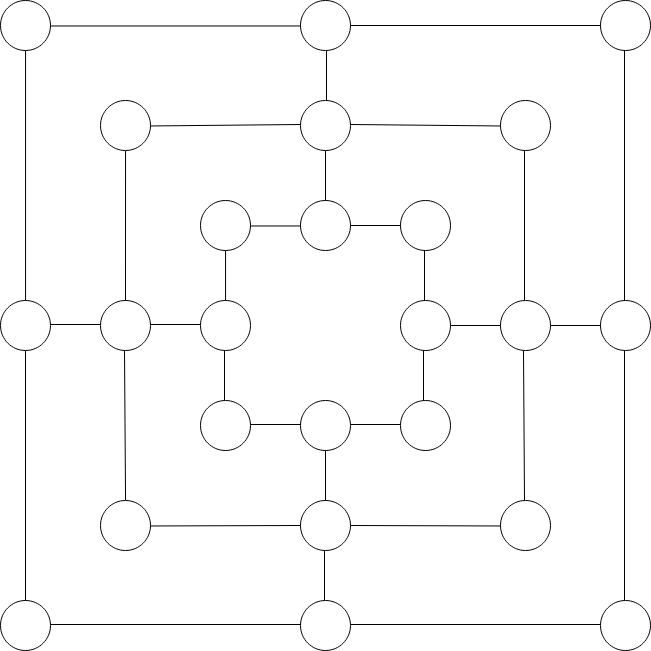
\includegraphics[width = 0.3\hsize]{figures/9MM_initial.png}
\caption{Board for Nine Men's Morris. The circles are the positions where the pawns can be placed or moved. Two positions are adjacent if there is an edge that links them.}
\label{fig:9MM_initial}
\end{figure}


\subsection{ASALTO}

\section{Representing Two-Players games in ASP}

\subsection{Similarities and Differences with Single-Player games}

%TODO source single player game
Representing Two-Players games in ASP follows the same scheme as for Single-Player games \cite{thielscher2009answer}. However, the predicate \texttt{role/1} needs to be modified to include the \textit{color} of each player. And the predicate \texttt{legal/3} has to take into account the fact that this is a turn-based game: a player has the right to play if and only if it is his turn.

\bigskip

Also, we will consider that each \textit{cell} has a set of coordinates (represented by the function \texttt{coord}), and a \textit{state}. For example, if the red player has a red pawn on the cell of coordinates $(1,3)$ at time $4$, then its translation in ASP is: \texttt{holds(cell(coord(1,3),red),4).}

\bigskip

For the moment, we only have studied single-phase game (in the background chapter, and in \cite{thielscher2009answer}). But \textit{Nine Men's Morris} and \textit{ASALTO} are two-phases games: in both of them, players place their pawns before moving them. So we need to define a new predicate \texttt{phase/2} that will appear in the bodies of the rules that define \texttt{legal/3}

\subsubsection{How to describe a two-players-game in ASP}

\begin{enumerate}

\item First, we describe the two players, by using \texttt{role/2}, that takes the name of the player as first argument, and his color for its second argument. From now on, we will suppose the two players are respectively called \textit{player1} and \textit{player2}.  

\item Also, we add the following rule: \newline
\texttt{opponent(P1, P2) :- role(P1, C1), role(P2, C2), P1 != P2.}

\item Then we describe the game as if it was a single player game with only one phase \citep{thielscher2009answer} (we forget that this is a turn based game with one or more phases). In particular, we will have to define the predicates \texttt{holds/3}, \texttt{legal/3}, \texttt{terminal/1}, and \texttt{wins/2}. Moreover,  \texttt{legal(P,M,T)} should only rely on \texttt{holds(C,T)} (at time T \textit{only}), \texttt{role/2}, and \texttt{opponent/2} for the moment. That way, \texttt{legal/3} does not depend on the previous actions or on the previous states, but only on the current states of the game.

\item In each rule that defines \texttt{legal/3} (of the form \texttt{legal(Player, a(X), T)}), we add the following predicate in the body: \texttt{can\_play(Player, a, T)}. This predicate is true if an only if \texttt{Player} has the right to perform an action of type \texttt{a} at time \texttt{T}. 

\item We define the predicate \texttt{can\_play/3}. For instance, in the case of the single-phase turn-based game, \texttt{can\_play/3} can be defined in the following way:\newline
\texttt{turn(player1, 1). }\\
\texttt{turn(P1, T+1) :- time(T), turn(P2, T), opponent(P1, P2).}\\
\texttt{can\_play(Player, Action, T) :- turn(Player, T).}


\item If the game has more than one phase, we need to describe the mechanism of the phase. At time $T=1$, we are in the first phase:\newline
\texttt{phase(phase(1), 1).}\\
We also want a phase to continue before it has finished:\newline
\texttt{phase(phase(N), T+1) :- time(T), phase(phase(N), T), not finished(phase(N), T+1).}\\
And if it has finished at time $T$, we go to the next phase:\newline
\texttt{phase(phase(N+1), T) :- time(T), finished(phase(N),T).}

\smallskip

Then, we add \texttt{phase/2} in the definition of \texttt{can\_play/3}. For example, if the two players can only play an action of type $a$ in the first phase, and of type $b$ in the second one, then it is equivalent to: \newline
\texttt{can\_play(Player, a, T) :- turn(Player, T), phase(phase(1),T).}\\
\texttt{can\_play(Player, b, T) :- turn(Player, T), phase(phase(2),T).}

\item Finally, we need to write the rules that define \texttt{finished/2}. These rules mainly depend on the board game: for \textit{Nine Men's Morris}, we move to the second phase once both players have placed all their pawns, but in \textit{ASALTO}, the soldiers are already positioned at time $T=1$, and only one player has to place the officers. 
\end{enumerate}

\subsection{Example: Nine Men's Morris in ASP}

\subsubsection{Coordinate System}

To represent \textit{Nine Men's Morris}, ASP, we first need to define what are the coordinates of the different cells. It seems that the system has three layers with the second one inside of the first one, and the third one inside the first one. This will be our second coordinate. Besides, there are eight cells in each layer. We will suppose the cell at the top-left corner of the layer has its first coordinate equal to 1, and we increment this coordinate as we go through the layer clockwise (Figure \ref{fig:9MM_coord}).

\begin{figure}[h]
\centering
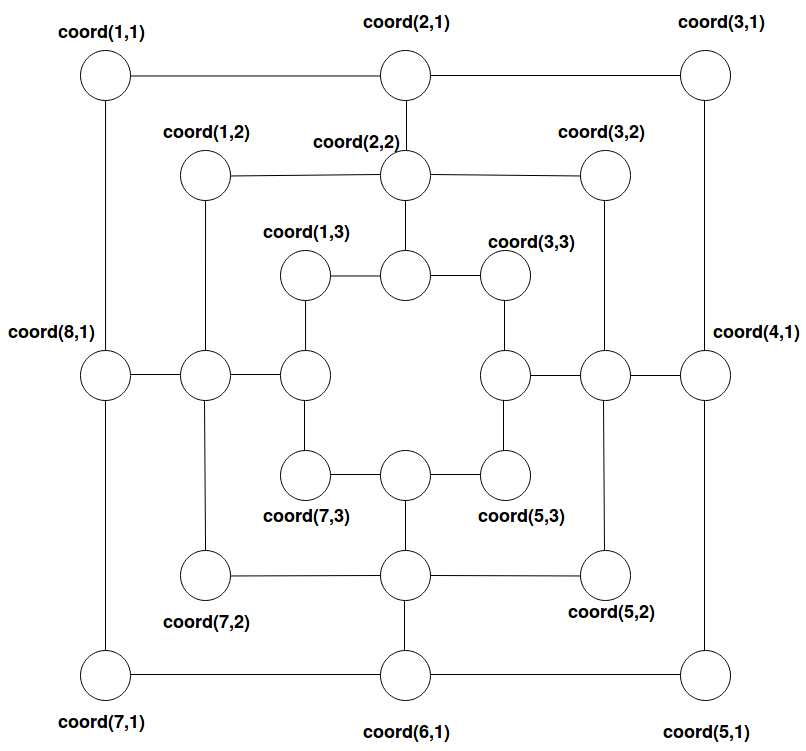
\includegraphics[width = 0.8\hsize]{figures/9MM_coord.png}
\caption{Coordinates of the cells used in Nine Men's Morris}
\label{fig:9MM_coord}
\end{figure}

\subsubsection{Nine Men's Morris described in ASP}

Here, each item refers to the last subsection.

\begin{enumerate}
\item First, we define the players and their roles\\
\texttt{role(player1, red).\\
role(player2, blue).\\}

\item We also add the following rule:\\
\texttt{opponent(P1, P2) :- role(P1, C1), role(P2, C2), P1 != P2.}

\item Here, we describe the game as in \cite{thielscher2009answer}: \texttt{legal/3} only depends on the state of the game (\texttt{holds/2}) and the player that is playing. In other words, we do not take the turn-based aspect into account.

\smallskip

%TODO : Appendix
We will only introduce quickly the predicates that were defined in the ASP Program. You may refer to the complete ASP program (in Appendix ??) for further information. 

%TODO : graph of dependancies.
\begin{tabular}{|c|c|}
\hline 
predicate & description \\ 
\hline
\hline 
\texttt{holds/3} & \makecell{Describes the state of the game: which cells are empty, \\ and which ones contain a pawn of color red or blue.} \\ 
\hline 
\texttt{legal/3} & \makecell{Tells which action a player has the right to perform\\ at a specific time. For instance, \texttt{legal(P,remove\_pawn(C),T)}\\ is true if and only if there is a pawn of the opponent \\in \texttt{C} and this pawn is not in a mill\\ (but if all his pawns form mills, the player \texttt{P} can still remove it)} \\ 
\hline 
\texttt{adjacent/2} & \makecell{Two pairs of coordinates are adjacent if there is an \\ edge that links them (Figure \ref{fig:9MM_coord})} \\ 
\hline 
\texttt{is\_in\_mill/2} & \makecell{\texttt{is\_in\_mill(Coord,mill(Coord\_1, Coord\_2, Coord\_3),T)} \\is true if a player owns the mill \texttt{mill(Coord\_1, Coord\_2, Coord\_3)} \\ and if \texttt{Coord} is one of its three coordinates} \\ 
\hline 
\texttt{has\_mill/3} & \makecell{\texttt{has\_mill(P,Mill,T)} is true if Mill is a mill owned \\by P at time T. It helps to define \texttt{is\_in\_mill/2}} \\ 
\hline 
\texttt{all\_in\_mill/2} & \makecell{Tells if a player has all his pawns in mills} \\ 
\hline 
\texttt{terminal/1} & \makecell{Represents the end of the game (when a player has won).\\ Its only argument is the time \texttt{T}.} \\ 
\hline 
\texttt{wins/2} & \makecell{Tells which player has won and when. \\ A player wins if the other has 2 or less pawns on the board\\ or if the other player is not able to perform any move.}  \\ 
\hline 
\texttt{pawns\_on\_board/3} & \makecell{Counts the number of pawns for each player on the board \\at each time. }\\ 
\hline 
\texttt{able\_to\_play/2} & \makecell{Tells if a player is able to perform any action at a specific time.} \\ 
\hline 
\end{tabular} 

\item After having defined \texttt{legal/3} in the previous step, we add:
\begin{itemize}
\item \texttt{can\_play(Player, place\_pawn, T)} in the body of \texttt{legal(Player, \\place\_pawn(Coord), T) }
\item \texttt{can\_play(Player, move, T)} in the body of \texttt{legal(Player, move(Coord\_1, Coord\_2), T) }
\item \texttt{can\_play(Player, remove\_pawn, T)} in the body of \texttt{legal(Player, \\remove\_pawn(Coord), T) }
\end{itemize}

\item 
We will consider that there are two phases in this game. In the first phase, the players place their respective pawns on the board. And in the second, they have finished to place their pawns and they only move them. 

\bigskip

We suppose that \texttt{player1} starts:
\texttt{can\_play(player1, place\_pawn, 1).} 

\bigskip

To define \texttt{can\_play/3} at time \texttt{T+1} we need to have a closer look at the rules of the game:

\begin{itemize}
\item A player can remove a pawn  at time \texttt{T} if he created a new mill with his action at time \texttt{T-1} (in both phases):\\
\texttt{can\_play(P1, remove\_pawn, T+1) :- does(P1, Action, T), time(T), has\_new\_mill(P1, T+1), role(P1, C1),  phase(phase(1..2),T+1).}
\item Thus, a player can place a pawn if his opponent did not get a new mill with his last action, and if the game is in its first phase:\\
\texttt{can\_play(P1, place\_pawn, T+1) :- does(P2, Action, T), time(T), not has\_new\_mill(P2, T+1), opponent\_player(P1, P2), phase(phase(1),T+1).}
\item Also, a player can move a pawn at time \texttt{T+1} if his opponent did not get a new mill at the same time, and if the game is in its second phase:\\ 
\texttt{can\_play(P1, move, T+1) :- does(P2, Action, T), time(T), \\not has\_new\_mill(P2, T+1), opponent\_player(P1, P2), phase(phase(2),T+1).}
\end{itemize}

The definition of \texttt{has\_new\_meal/2} can be found in appendix ??

\item As there are more than one phase, we add the following definition of \texttt{phase/2} in the program (as explained in the last subsection):\\
\texttt{phase(phase(1), 1).}\\
\texttt{phase(phase(N), T+1) :- time(T), phase(phase(N), T),\\ not finished(phase(N), T+1).}\\
\texttt{phase(phase(N+1), T) :- time(T), finished(phase(N),T).}

\item Finally we define the predicate \texttt{finished/2}:
\begin{itemize}
\item The first phase is finished when both players do not have any pawn in their hands: \\
\texttt{finished(phase(1), T) :- time(T), has\_pawns(player1, 0, T), \\has\_pawns(player2, 0, T).}\\
Where \texttt{has\_pawns/3} counts the number of pawns that each player still has to place. Its complete definition may be found in appendix ??
%TODO : faire une recherche sur le latex pour les ?? et les remplacer
\item We suppose that the second phase never finishes (as there is no third phase). So we do not need to define \texttt{finished(phase(2), T)}. 
\end{itemize}

\end{enumerate}




% tableau: gauche -> règle en anglais, droite -> rule en ASP

%%%%%%%%%%%%%%%%%%%%%%%%%%%%%%%%%%%%
\chapter{Learning rules for board Games}

\section{General Idea}

We observe people playing the game, and \\
if they do a valid action - positive example\\
if they do an action that is not legal - negative example\\

\bigskip

goal : learning legal/3 predicate (according to the structure of GDL)

\bigskip

source:  has been made in ILASP (paper reference)%(or concurrent) papers 

\bigskip

Learning predicate wins/2 ?

\section{Evaluation}

Evaluation at least for Five Field Kono.

\bigskip

\begin{tabular}{|c|c|c|}
\hline 
added example & hypothesis found & time (s) \\ 
\hline 
\hline
• & • & • \\ 
\hline 
• & • & • \\ 
\hline 
\end{tabular} 

%%%%%%%%%%%%%%%%%%%%%%%%%%%%%%%%%%%%
\chapter{Learning strategies}

% 

For the moment, we only have implemented the \textit{tic-tac-toe} and the \textit{Field Field Kono} in python by using \texttt{pygame} (python library for video games).
%TODO : reference pygame
\smallskip

The idea would be to learn from the actions performed by a player to train our system by using ILASP. Then we could make him play against this trained system and continue to train it that way.

\section{First Method: maximize the chances of winning}
%TODO : Change title ?

\subsection{Learning Exception Structure}

Supposing we are at time $T=t$, we want the computer to induce a set of rules $H$ such that:
\begin{itemize}
\item There is a move $m$ such that for every answer set $A$ of $B\cup H,\:  does(player1, m, t)\in A$
\item For every answer set $A$ of $B\cup H$, for all move $m_1$ different from $m$, we have: $does(player1, m_1, t) \notin A$
\item $H$ also tries to take into account the possible future moves.
\end{itemize}

To reduce the hypothesis space, it would be interesting to focus only on \textit{exception structures}, which means we want $H$ to be of this form:
\[H=
\begin{Bmatrix}
\texttt{does(player1, move\_p1\_t0\_1, t).}\\
\texttt{does(player1, move\_p1\_t2\_1, t+2) :- \textcolor{red}{does(player2, move\_p2\_t1\_1, t+1)}.}\\
\texttt{does(player1, move\_p1\_t2\_2, t+2) :- not \textcolor{red}{does(player2, move\_p2\_t1\_1, t+1)}.} 
\end{Bmatrix}
\]
%TODO : A FAIRE avec le cours de Marek Sergot ???
In the set above, we will call "\textit{exception rule}" the second rule, and "\textit{general rule}" the third.

\begin{remark}
 The hypothesis space could also be extended so that it accepts two or more  exception rules.
\[H=
\begin{Bmatrix}
\texttt{does(player1, move\_p1\_t0\_1, t).}\\
\texttt{does(player1, move\_p1\_t2\_1, t+2) :-} &\texttt{\textcolor{red}{does(player2, move\_p2\_t1\_1, t+1)}.}\\
\texttt{does(player1, move\_p1\_t2\_2, t+2) :-} &\texttt{\textcolor{blue}{does(player2, move\_p2\_t1\_2, t+1)}.}\\
\texttt{does(player1, move\_p1\_t2\_3, t+2) :-} &\texttt{not \textcolor{red}{does(player2, move\_p2\_t1\_1, t+1)},}\\ &\texttt{not \textcolor{blue}{does(player2, move\_p2\_t1\_2, t+1)}.} 
\end{Bmatrix}
\]
\end{remark}

%TODO : Deuxième remarque pour expliquer comment prendre en compte ce qu'il se passe à t+4 ?

Moreover, the atoms in the exception rule must appear in the general rule (see the \textcolor{red}{red} and \textcolor{blue}{blue} atoms in the hypotheses above).

\bigskip

%TODO : good version of ILASP ?
With ILASP 3.1.0 it is possible add "bias constraints" to specify what kind of rule we want to learn. However it is not possible to add constraints on the whole set of rules induced. As a consequence, we cannot say that for every solution $H$ in $ILP_{LAS}(B,S_M,E^+,E^-)$, 
if there are $move\_p1\_t2\_1$ and $move\_p2\_t1\_1$ such that:
\\ $\texttt{"does(player1,move\_p1\_t2\_1,t+2) :- \textcolor{red}{does(player2,move\_p2\_t1\_1,t+1)}."}\in H$, 
then there is $move\_p1\_t2\_2$ such that:\\
$\texttt{"does(player1,move\_p1\_t2\_2,t+2):- not \textcolor{red}{does(player2,move\_p2\_t1\_1,t+1)}."}\in H$

\bigskip

The solution we used consists in using the ASPAL encoding in ILASP. With this encoding, we can add more flexible constraints for the hypothesis space.

\subsection{Example}

\paragraph{Current State of the Game}

Consider a tic-tac-toe game after the 4 following moves (represented in \ref{fig:ttt_ex}):\newline
\texttt{does(player1, fill(coord(2,2)),1).\\
does(player2, fill(coord(1,2)),2).\\
does(player1, fill(coord(1,1)),3).\\
does(player2, fill(coord(3,3)),4).}

\begin{figure}[h]
\centering
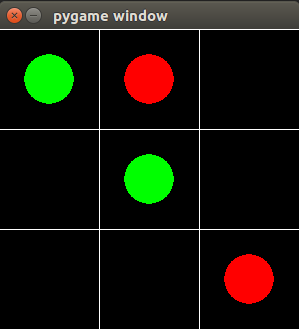
\includegraphics[width = 0.3\hsize]{figures/ttt_example.png}
\caption{State of a tic-tac-toe game after 4 moves. The green player plays first (he is \texttt{player1}).}
\label{fig:ttt_ex}
\end{figure}

Here, we are the green player and we want to find a move such that we are sure to win in three moves.

\paragraph{Hypothesis space}

We use the following mode declaration:
\[ M=
\begin{Bmatrix} 
m1 :& \texttt{modeh(does(player1,\#move,5)).} \\ 
m2 :& \texttt{modeh(does(player1,\#move,7)).}\\
m3 :& \texttt{modeb(does(player2,\#move,6)).}\\
m4 :& \texttt{modeb(not does(player2,\#move,6)).}
\end{Bmatrix}
\]
%TODO : explain how a mode declaration works OR reference to an article to explain it

Moreover, we take the following hypothesis space:
\[ R_M=
\begin{Bmatrix}
\texttt{does(player1, X, 5).} \\ 
\texttt{does(player1, Z, 7) :-} & \texttt{does(player2, Y, 6).}\\
\texttt{does(player1, X, 7) :-}  & \texttt{not does(player2, Y, 6).}
\end{Bmatrix}
\]

So the top theory that we use for this example is:
\[ T=
\begin{Bmatrix}
\texttt{does(player1, X, 5) :-} & \texttt{legal(player1,X,5), rule((m1),(X)).} \\ 

\texttt{does(player1, Z, 7) :-} & \texttt{legal(player1, Z, 7), legal(player2, Y, 6), }\\ 
 & \texttt{does(player2, Y, 6), rule((m2,m3,2),(Z,Y)).} \\

\texttt{does(player1, X, 7) :-} & \texttt{legal(player1, X, 7), legal(player2, Y, 6), } \\
& \texttt{not does(player2, Y, 6), rule((m2,m4,2),(X,Y)).}
\end{Bmatrix}
\]
where we added the predicate \texttt{legal/3} to make the variables safe.

\bigskip

So now the hypothesis we want to learn with ILASP has the following form:
\[H=
\begin{Bmatrix}
\texttt{rule((m1),(\#move\_p1\_t0\_1)).}\\
\texttt{rule((m2,m3,2),(\#move\_p1\_t2\_1, \#move\_p2\_t1\_1))}.\\
\texttt{rule((m2,m4,2),(\#move\_p1\_t2\_2, \#move\_p2\_t1\_1))}.
\end{Bmatrix}
\]

\bigskip

We want $H$ to contain only one rule of each type: only one rule of the form\\ \texttt{rule((m1),(\#move\_p1\_t0\_1))} and so on... 
So we add some rules to make them unique:\newline
\texttt{rule1 :- rule((m1),(fill(coord(X,Y)))).}\\
\texttt{:- not rule1.}\\
\texttt{:- rule((m1),(fill(coord(X1,Y1)))), rule((m1),(fill(coord(X2,Y2)))), g(X1, Y1)< g(X2, Y2). }\\

\smallskip

The two first rules make \texttt{rule((m1),(\#move\_p1\_t0\_1))} appear at least once, and the last rule makes it appear at most once. We add similar rules for \texttt{rule((m2,m3,2), (\#move\_p1\_t2\_1, \#move\_p2\_t1\_1))} and \texttt{rule((m2,m4,2), (\#move\_p1\_t2\_2, \#move\_p2\_t1\_1))}.

\bigskip

Also, we added some constraints to reduce the computation time. For instance, if \texttt{rule((m1),(fill(coord(X,Y))))} is true, then \texttt{legal(player1,fill(coord(X,Y)),5)} must be true. So we add the following constraint:\newline
\texttt{:- rule((m1),(fill(coord(X,Y)))), not legal(player1,fill(coord(X,Y)),5).}

\bigskip

And if \texttt{rule((m2,m4,2),(fill(coord(X,Y)),fill(coord(Z,T))))} and \texttt{not does(player2, fill(coord(Z,T)), 6)} are true, then \texttt{legal(player1, fill(coord(X,Y)),7)} must be true unless \texttt{player2} plays in \texttt{coord(X,Y)} at time 6. Thus, we add the following constraint:\newline
\texttt{:- rule((m2,m4,2),(fill(coord(X,Y)),fill(coord(Z,T)))), not does(player2, fill(coord(Z,T)), 6),}
\texttt{ not legal(player1, fill(coord(X,Y)),7).}\newline
and we add this context-dependent example to the set of positive examples : \newline
$<<\{\texttt{wins(player2,8)}\},\emptyset>,\\ \{\texttt{:- rule((m2,m4,2),(fill(coord(X,Y)),fill(coord(Z,T)))),} \\ \texttt{not does(player2, fill(coord(X,Y)), 6).}\}>$
%TODO : change fonts to textt in partial interpretations

\smallskip

With this example, we are sure that there will be at least one answer set where \texttt{player2} plays in \texttt{coord(X,Y)}.


\paragraph{Declaring the examples}

First of all, we want the first player to win in two moves all the time. So there is no answer set that does not contain \texttt{wins(player1,8)}. Thus, we take : $E^-=\{<\emptyset,\{\texttt{wins(player1,8)}\}>\}$.

\bigskip

For the positive examples, we only need to take the one given in the previous paragraph. The \texttt{wins(player2,8)} in it is optional but it reduces the computation time from 11 seconds to 1 second.

\paragraph{Evaluation}

%TODO : to complete

\subsection{Finding a move in the middle of a game}

We are only able to look two moves ahead, so we cannot predict how to win a game if we are not very close to the end. It would be a good idea to define what a good state is (or to make ILASP learn it). And after that, it could be possible to choose a state at time $t$ that maximizes the chances of reaching a good state at time $t+2$.

\bigskip

For instance, if we consider the game represented in figure \ref{fig:graph_game}, where \texttt{player1} plays at times $t$ and $t+2$ and \texttt{player2} plays at time $t+1$. 

\smallskip

We want to maximize the probability of reaching a good state at $t+2$. So we choose $a(x)$ such that $\#\{b(y)|legal(b(y))\wedge\:\left( b(y) \implies \exists \:c(z) \:;\: legal(c(z)) \wedge good\_state(state\_c(z)) \right)\}$ is maximal, which is $a(1)$ in this example.

\begin{figure}[h]
\centering
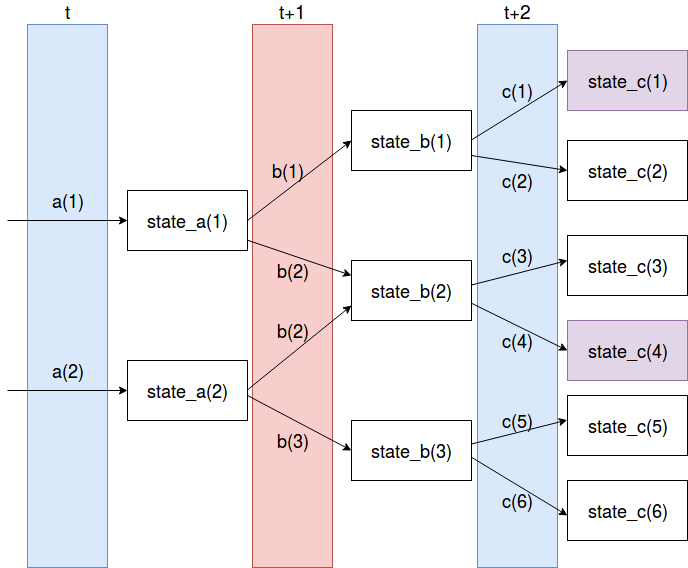
\includegraphics[width = 0.8\hsize]{figures/graph_game.png}
\caption{Desription of a graph game with its states and the actions to perform to go from one state to another. The blue player (that plays at times $t$ and $t+2$) is \texttt{player1}. The states in purple are the good states.}
\label{fig:graph_game}
\end{figure}

\section{Second Method: recognize preferred moves and states}

Goal: learn the preferences of the player by using Weak Constraints.

\subsection{Learning what kind of action the player prefers}

\emph{When we have the choice of the kind of action like in Five Field Kono : Learning  direction, up\_right, down\_right... }

%TODO : not very interesting isn't it ? cos' it could be done just by counting them.

\subsection{Discover the sates of the board that the player chooses}

Talk about the the drawbacks of last subsection: does not give enough information. So now we learn what kind of configuration the player prefers in a game. 

%TODO : parler des limitations de la section précédente.
% certes on pourrait lier les deux: does() :- holds(), holds(),...
% Mais serait trop computationally expensive ???

\subsubsection{How to represent patterns}

How to represent patterns, how to combine them. Example of Five Field Kono

% 

\subsubsection{Learning preferred patterns}

Test results with program, with time results.

Problem: one simple pattern can cover many more complex patterns

%%%%%%%%%%%%%%%%%%%%%%%%%%%%%%%%%%%%




\chapter{Evaluation}

TODO : or maybe a part evaluation in each of the previous chapters

\chapter{Conclusions and Future work}


\begin{comment}

\chapter{Progress}

\section{Two-Players games}

\subsection{Representing Two-Players games in ASP}

We only need to change a few things to adapt the rules in single-player games for two-players games:
\begin{itemize}
\item First of all, we create two roles instead of one:\\ \texttt{role(player1).}\\
\texttt{role(player2).}
\item Then we replace \texttt{player} in every rule by the variable \texttt{P}, and we add \texttt{role(P)} at the end of each rule.
\item Besides, only one move is allowed at each time step:\\
\texttt{1\{does(P,M,T):role(P),move\_domain(M)\}1 :- not terminated(T).}\\
\texttt{move\_domain(go(left))}.\\
\texttt{move\_domain(go(right))}.

\item Finally, a player cannot play twice:\\
\texttt{:- does(P,M1,T), does(P,M2,T+1).}

\end{itemize}

\subsection{Games under study}

This project focuses on three games: \textit{Five Field Kono}, \textit{Nine Men's Morris} and \textit{ASALTO}.

%TODO : give references

\smallskip

For the moment, we have only tried to study how to learn a strategy on a very simple game (with a small number of possible states): the \textit{tic-tac-toe}. Afterwards, we will try to extend what we have done on \textit{tic-tac-toe} to \textit{Five Field Kono}.

\smallskip

Moreover, we have represented these four games in ASP.

\section{Finding/Learning a strategy}

We found several ways of thinking about how to learn a strategy:
\begin{itemize}
\item The first one consists in trying to find a move such that: whatever the second player does the next turn (or his 2 or 3 next turns), the first player can still win. This method seems very similar to the \textit{minimax} algorithm. 
\item We could also study several games played by two players, and try to make hypotheses about what to do in which circumstances. 
\item It is possible to imagine a mix between the two previous methods: the second one tells us what are the good states, and the first method gives us a move so that we can reach a good state for sure (whatever the second player does).
\end{itemize}

For the moment, we have only studied the first method.

%TODO : give references (minimax)
%TODO : parler des inconvénients de chaque méthode.

\subsection{Planning moves}

\subsubsection{Basic method}

In \textit{tic-tac-toe}, we initialized the game with 4 specific moves already done. If we restrict the hypothesis space by not allowing negation by failure nor constraints, ILASP can find some (ground) hypotheses of the form:\\
\texttt{does(player1,fill(cell(x)),5). \% at time T=5 } \\
\texttt{does(player1,fill(cell(y)),7) :- does(player2,fill(cell(z)),6).}\\
that make \texttt{player1} win. 

\smallskip

For this, we only need to specify that the program has at least an answer set: \texttt{\#pos(\{\},\{\})}, and that \texttt{player1} wins in every answer set: \texttt{\#neg(\{\},\{wins(player1)\})}.

\subsubsection{Problem with negation by failure}



\subsubsection{Solution Found for the Graph Games}


%%%%%%%%%%%%%%%%%%%%%%%%%%%%%%%%%%%%
%*%\chapter{Experimental Results}


%%%%%%%%%%%%%%%%%%%%%%%%%%%%%%%%%%%%

\end{comment}

%% bibliography
\bibliographystyle{alpha}
\bibliography{bibli}

\appendix


%TODO : make it clearer with stuff like this to present the predicates:
%%%%%%%%%%%%%%%%%%%
% COUCOU%%%%%%%%%%%
%%%%%%%%%%%%%%%%%%%
\chapter{Nine Men's Morris described in ASP}

\VerbatimInput[label=\fbox{\color{Black}Nine Men's Morris}]{9MM.lp}

\end{document}
